\documentclass{article}
\usepackage{graphicx}

\begin{document}

\centerline{\Large \bf LAMMPS Developer Guide}
\centerline{\bf 23 Aug 2011}

\vspace{0.5in}

This document is a developer guide to the LAMMPS molecular dynamics
package, whose WWW site is at lammps.sandia.gov.  It describes the
internal structure and algorithms of the code.  Sections will be added
as we have time, and in response to requests from developers and
users.

\tableofcontents

\pagebreak
\section{LAMMPS source files}

LAMMPS source files are in two directories of the distribution
tarball.  The src directory has the majority of them, all of which are
C++ files (*.cpp and *.h).  Many of these files are in the src
directory itself.  There are also dozens of ``packages'', which can be
included or excluded when LAMMPS is built.  See the
doc/Section\_build.html section of the manual for more information
about packages, or type ``make'' from within the src directory, which
lists package-related commands, such as ``make package-status''.  The
source files for each package are in an all-uppercase sub-directory of
src, like src/MOLECULE or src/USER-CUDA.  If the package is currently
installed, copies of the package source files will also exist in the
src directory itself.  The src/STUBS sub-directory is not a package
but contains a dummy version of the MPI library, used when building a
serial version of the code.

The lib directory also contains source code for external libraries,
used by a few of the packages.  Each sub-directory, like meam or gpu,
contains the source files, some of which are in different languages
such as Fortran.  The files are compiled into libraries from within
each sub-directory, e.g. performing a ``make'' in the lib/meam directory
creates a libmeam.a file.  These libraries are linked to during a
LAMMPS build, if the corresponding package is installed.

LAMMPS C++ source files almost always come in pairs, such as run.cpp
and run.h.  The pair of files defines a C++ class, the Run class in
this case, which contains the code invoked by the ``run'' command in a
LAMMPS input script.  As this example illustrates, source file and
class names often have a one-to-one correspondence with a command used
in a LAMMPS input script.  Some source files and classes do not have a
corresponding input script command, e.g. ``force.cpp'' and the Force
class.  They are discussed in the next section.

\pagebreak
\section{Class hierarchy of LAMMPS}

Though LAMMPS has a lot of source files and classes, its class
hierarchy is quite simple, as outlined in Fig \ref{fig:classes}.  Each
boxed name refers to a class and has a pair of associated source files
in lammps/src, e.g. ``memory.cpp'' and ``memory.h''.  More details on the
class and its methods and data structures can be found by examining
its *.h file.

LAMMPS (lammps.cpp/h) is the top-level class for the entire code.  It
holds an ``instance'' of LAMMPS and can be instantiated one or more
times by a calling code.  For example, the file src/main.cpp simply
instantiates one instance of LAMMPS and passes it the input script.

The file src/library.cpp contains a C-style library interface to the
LAMMPS class.  See the lammps/couple and lammps/python directories for
examples of simple programs that use LAMMPS through its library
interface.  A driver program can instantiate the LAMMPS class multiple
times, e.g. to embed several atomistic simulation regions within a
mesoscale or continuum simulation domain.

There are a dozen or so top-level classes within the LAMMPS class that
are visible everywhere in the code.  They are shaded blue in Fig
\ref{fig:classes}.  Thus any class can refer to the y-coordinate of
local atom $I$ as atom$\rightarrow$x[i][1].  This visibility is
enabled by a bit of cleverness in the Pointers class (see
src/pointers.h) which every class inherits from.

There are a handful of virtual parent classes in LAMMPS that define
what LAMMPS calls ``styles''.  They are shaded red in Fig
\ref{fig:classes}.  Each of these are parents of a number of child
classes that implement the interface defined by the parent class.  For
example, the fix style has around 100 child classes.  They are the
possible fixes that can be specified by the fix command in an input
script, e.g. fix nve, fix shake, fix ave/time, etc.  The corresponding
classes are Fix (for the parent class), FixNVE, FixShake, FixAveTime,
etc.  The source files for these classes are easy to identify in the
src directory, since they begin with the word ``fix'', e,g,
fix\_nve.cpp, fix\_shake,cpp, fix\_ave\_time.cpp, etc.

The one exception is child class files for the ``command'' style.  These
implement specific commands in the input script that can be invoked
before/after/between runs or which launch a simulation.  Examples are
the create\_box, minimize, run, and velocity commands which encode the
CreateBox, Minimize, Run, and Velocity classes.  The corresponding
files are create\_box,cpp, minimize.cpp, run.cpp, and velocity.cpp.
The list of command style files can be found by typing ``grep
COMMAND\_CLASS *.h'' from within the src directory, since that word in
the header file identifies the class as an input script command.
Similar words can be grepped to list files for the other LAMMPS
styles.  E.g. ATOM\_CLASS, PAIR\_CLASS, BOND\_CLASS, REGION\_CLASS,
FIX\_CLASS, COMPUTE\_CLASS, DUMP\_CLASS, etc.

\begin{figure}[htb]
 \begin{center}
 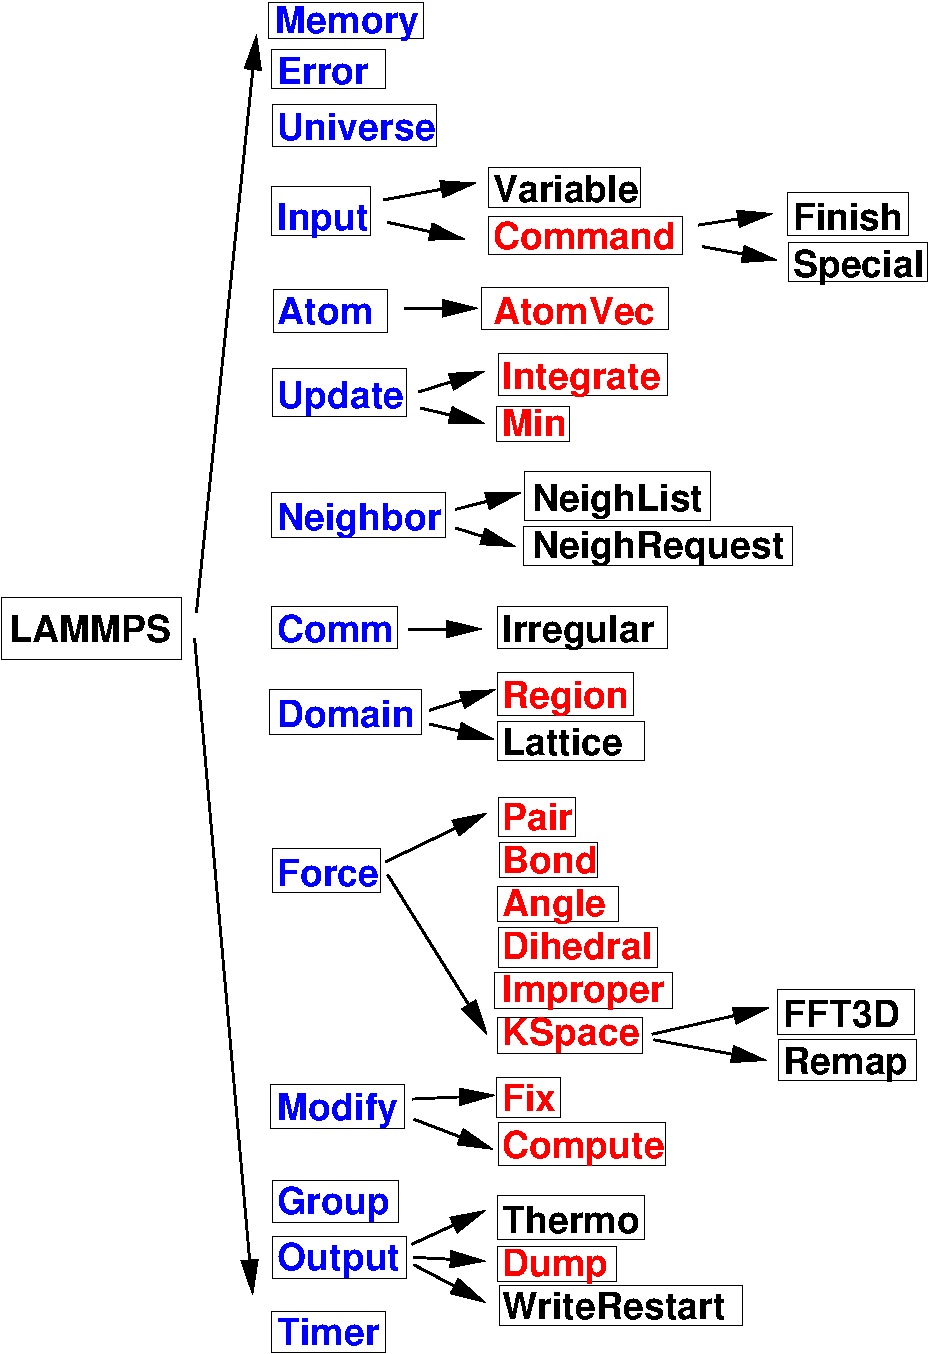
\includegraphics[height=4in]{classes.pdf}
 \end{center}
 \caption{Class hierarchy within LAMMPS source code.}
\label{fig:classes}
\end{figure}

More details on individual classes in Fig \ref{fig:classes} are as
follows:

\begin{itemize}

\item The Memory class handles allocation of all large vectors and
  arrays.

\item The Error class prints all error and warning messages.

\item The Universe class sets up partitions of processors so that
  multiple simulations can be run, each on a subset of the processors
  allocated for a run, e.g. by the mpirun command.

\item The Input class reads an input script, stores variables, and
  invokes stand-alone commands that are child classes of the Command
  class.

\item As discussed above, the Command class is a parent class for
  certain input script commands that perform a one-time operation
  before/after/between simulations or which invoke a simulation.  They
  are instantiated from within the Input class, invoked, then
  immediately destructed.

\item The Finish class is instantiated to print statistics to the
  screen after a simulation is performed, by commands like run and
  minimize.

\item The Special class walks the bond topology of a molecular system
  to find 1st, 2nd, 3rd neighbors of each atom.  It is invoked by
  several commands, like read\_data, read\_restart, and replicate.

\item The Atom class stores all per-atom arrays.  More precisely, they
  are allocated and stored by the AtomVec class, and the Atom class
  simply stores a pointer to them.  The AtomVec class is a parent
  class for atom styles, defined by the atom\_style command.

\item The Update class holds an integrator and a minimizer.  The
  Integrate class is a parent style for the Verlet and rRESPA time
  integrators, as defined by the run\_style input command.  The Min
  class is a parent style for various energy minimizers.

\item The Neighbor class builds and stores neighbor lists.  The
  NeighList class stores a single list (for all atoms).  The
  NeighRequest class is called by pair, fix, or compute styles when
  they need a particular kind of neighbor list.

\item The Comm class performs interprocessor communication, typically
  of ghost atom information.  This usually involves MPI message
  exchanges with 6 neighboring processors in the 3d logical grid of
  processors mapped to the simulation box.  Sometimes the Irregular
  class is used, when atoms may migrate to arbitrary processors.

\item The Domain class stores the simulation box geometry, as well as
  geometric Regions and any user definition of a Lattice.  The latter
  are defined by region and lattice commands in an input script.

\item The Force class computes various forces between atoms.  The Pair
  parent class is for non-bonded or pair-wise forces, which in LAMMPS
  lingo includes many-body forces such as the Tersoff 3-body
  potential.  The Bond, Angle, Dihedral, Improper parent classes are
  styles for bonded interactions within a static molecular topology.
  The KSpace parent class is for computing long-range Coulombic
  interactions.  One of its child classes, PPPM, uses the FFT3D and
  Remap classes to communicate grid-based information with neighboring
  processors.

\item The Modify class stores lists of Fix and Compute classes, both
  of which are parent styles.

\item The Group class manipulates groups that atoms are assigned to
  via the group command.  It also computes various attributes of
  groups of atoms.

\item The Output class is used to generate 3 kinds of output from a
  LAMMPS simulation: thermodynamic information printed to the screen
  and log file, dump file snapshots, and restart files.  These
  correspond to the Thermo, Dump, and WriteRestart classes
  respectively.  The Dump class is a parent style.

\item The Timer class logs MPI timing information, output at the end
  of a run.

\end{itemize}

%%\pagebreak
%%\section{Spatial decomposition and parallel operations}
%%distributed memory
%%Ref to JCP paper
%%diagram of 3d grid of procs and spatial decomp
%%6-way comm
%%ghost atoms, PBC added when comm (in atom class)

%%\pagebreak
%%\section{Fixes, computes, variables}
%%fixes intercolate in timestep, store per-atom info
%%computes based on current snapshot
%%equal- and atom-style variables
%%output they produce - see write-up in HowTo

\pagebreak
\section{How a timestep works}

The first and most fundamental operation within LAMMPS to understand
is how a timestep is structured.  Timestepping is performed by the
Integrate class within the Update class.  Since Integrate is a parent
class, corresponding to the run\_style input script command, it has
child classes.  In this section, the timestep implemented by the
Verlet child class is described.  A similar timestep is implemented by
the Respa child class, for the rRESPA hierarchical timestepping
method.  The Min parent class performs energy minimization, so does
not perform a literal timestep.  But it has logic similar to what is
described here, to compute forces and invoke fixes at each iteration
of a minimization.  Differences between time integration and
minimization are highlighted at the end of this section.

The Verlet class is encoded in the src/verlet.cpp and verlet.h files.
It implements the velocity-Verlet timestepping algorithm.  The
workhorse method is Verlet::run(), but first we highlight several
other methods in the class.

\begin{itemize}

\item The init() method is called at the beginning of each dynamics
  run.  It simply sets some internal flags, based on user settings in
  other parts of the code.

\item The setup() or setup\_minimal() methods are also called before
  each run.  The velocity-Verlet method requires current forces be
  calculated before the first timestep, so these routines compute
  forces due to all atomic interactions, using the same logic that
  appears in the timestepping described next.  A few fixes are also
  invoked, using the mechanism described in the next section.  Various
  counters are also initialized before the run begins.  The
  setup\_minimal() method is a variant that has a flag for performing
  less setup.  This is used when runs are continued and information
  from the previous run is still valid.  For example, if repeated
  short LAMMPS runs are being invoked, interleaved by other commands,
  via the ``pre no'' and ``every'' options of the run command, the
  setup\_minimal() method is used.

\item The force\_clear() method initializes force and other arrays to
  zero before each timestep, so that forces (torques, etc) can be
  accumulated.

\end{itemize}

Now for the Verlet::run() method.  Its structure in hi-level pseudo
code is shown in Fig \ref{fig:verlet}.  In the actual code in
src/verlet.cpp some of these operations are conditionally invoked.

\begin{figure}[htb]
 \begin{center}
 \begin{verbatim}
loop over N timesteps:
  ev_set()

  fix->initial_integrate()
  fix->post_integrate()

  nflag = neighbor->decide()
  if nflag:
    fix->pre_exchange()
    domain->pbc()
    domain->reset_box()
    comm->setup()
    neighbor->setup_bins()
    comm->exchange()
    comm->borders()
    fix->pre_neighbor()
    neighbor->build()
  else
    comm->forward_comm()

  force_clear()
  fix->pre_force()

  pair->compute()
  bond->compute()
  angle->compute()
  dihedral->compute()
  improper->compute()
  kspace->compute()

  comm->reverse_comm()

  fix->post_force()
  fix->final_integrate()
  fix->end_of_step()

  if any output on this step: output->write()
  \end{verbatim}
 \end{center}
 \caption{Pseudo-code for the Verlet::run() method.}
\label{fig:verlet}
\end{figure}

The ev\_set() method (in the parent Integrate class), sets two flags
({\em eflag} and {\em vflag}) for energy and virial computation.  Each
flag encodes whether global and/or per-atom energy and virial should
be calculated on this timestep, because some fix or variable or output
will need it.  These flags are passed to the various methods that
compute particle interactions, so that they can skip the extra
calculations if the energy and virial are not needed.  See the
comments with the Integrate::ev\_set() method which document the flag
values.

At various points of the timestep, fixes are invoked,
e.g. fix$\rightarrow$initial\_integrate().  In the code, this is
actually done via the Modify class which stores all the Fix objects
and lists of which should be invoked at what point in the timestep.
Fixes are the LAMMPS mechanism for tailoring the operations of a
timestep for a particular simulation.  As described elsewhere
(unwritten section), each fix has one or more methods, each of which
is invoked at a specific stage of the timestep, as in Fig
\ref{fig:verlet}.  All the fixes defined in an input script with an
initial\_integrate() method are invoked at the beginning of each
timestep.  Fix nve, nvt, npt are examples, since they perform the
start-of-timestep velocity-Verlet integration to update velocities by
a half-step, and coordinates by a full step.  The post\_integrate()
method is next.  Only a few fixes use this, e.g. to reflect particles
off box boundaries in the FixWallReflect class.

The decide() method in the Neighbor class determines whether neighbor
lists need to be rebuilt on the current timestep.  If not, coordinates
of ghost atoms are acquired by each processor via the forward\_comm()
method of the Comm class.  If neighbor lists need to be built, several
operations within the inner if clause of Fig \ref{fig:verlet} are
first invoked.  The pre\_exchange() method of any defined fixes is
invoked first.  Typically this inserts or deletes particles from the
system.

Periodic boundary conditions are then applied by the Domain class via
its pbc() method to remap particles that have moved outside the
simulation box back into the box.  Note that this is not done every
timestep. but only when neighbor lists are rebuilt.  This is so that
each processor's sub-domain will have consistent (nearby) atom
coordinates for its owned and ghost atoms.  It is also why dumped atom
coordinates can be slightly outside the simulation box.

The box boundaries are then reset (if needed) via the reset\_box()
method of the Domain class, e.g. if box boundaries are shrink-wrapped
to current particle coordinates.  A change in the box size or shape
requires internal information for communicating ghost atoms (Comm
class) and neighbor list bins (Neighbor class) be updated.  The
setup() method of the Comm class and setup\_bins() method of the
Neighbor class perform the update.

The code is now ready to migrate atoms that have left a processor's
geometric sub-domain to new processors.  The exchange() method of the
Comm class performs this operation.  The borders() method of the Comm
class then identifies ghost atoms surrounding each processor's
sub-domain and communicates ghost atom information to neighboring
processors.  It does this by looping over all the atoms owned by a
processor to make lists of those to send to each neighbor processor.
On subsequent timesteps, the lists are used by the
Comm::forward\_comm() method.

Fixes with a pre\_neighbor() method are then called.  These typically
re-build some data structure stored by the fix that depends on the
current atoms owned by each processor.

Now that each processor has a current list of its owned and ghost
atoms, LAMMPS is ready to rebuild neighbor lists via the build()
method of the Neighbor class.  This is typically done by binning all
owned and ghost atoms, and scanning a stencil of bins around each
owned atom's bin to make a Verlet list of neighboring atoms within the
force cutoff plus neighbor skin distance.

In the next portion of the timestep, all interaction forces between
particles are computed, after zeroing the per-atom force vector via
the force\_clear() method.  If the newton flag is set to ``on'' by the
newton command, forces on both owned and ghost atoms are calculated.

Pairwise forces are calculated first, which enables the global virial
(if requested) to be calculated cheaply (at the end of the
Pair::compute() method), by a dot product of atom coordinates and
forces.  By including owned and ghost atoms in the dot product, the
effect of periodic boundary conditions is correctly accounted for.
Molecular topology interactions (bonds, angles, dihedrals, impropers)
are calculated next.  The final contribution is from long-range
Coulombic interactions, invoked by the KSpace class.

If the newton flag is on, forces on ghost atoms are communicated and
summed back to their corresponding owned atoms.  The reverse\_comm()
method of the Comm class performs this operation, which is essentially
the inverse operation of sending copies of owned atom coordinates to
other processor's ghost atoms.

At this point in the timestep, the total force on each atom is known.
Additional force constraints (external forces, SHAKE, etc) are applied
by Fixes that have a post\_force() method.  The second half of the
velocity-Verlet integration is then performed (another half-step
update of the velocities) via fixes like nve, nvt, npt.

At the end of the timestep, fixes that define an end\_of\_step()
method are invoked.  These typically perform a diagnostic calculation,
e.g. the ave/time and ave/spatial fixes.  The final operation of the
timestep is to perform any requested output, via the write() method of
the Output class.  There are 3 kinds of LAMMPS output: thermodynamic
output to the screen and log file, snapshots of atom data to a dump
file, and restart files.  See the thermo\_style, dump, and restart
commands for more details.

The iteration performed by an energy minimization is similar to the
dynamics timestep of Fig \ref{fig:verlet}.  Forces are computed,
neighbor lists are built as needed, atoms migrate to new processors,
and atom coordinates and forces are communicated to neighboring
processors.  The only difference is what Fix class operations are
invoked when.  Only a subset of LAMMPS fixes are useful during energy
minimization, as explained in their individual doc pages.  The
relevant Fix class methods are min\_pre\_exchange(),
min\_pre\_force(), and min\_post\_force().  Each is invoked at the
appropriate place within the minimization iteration.  For example, the
min\_post\_force() method is analogous to the post\_force() method for
dynamics; it is used to alter or constrain forces on each atom, which
affects the minimization procedure.

\pagebreak
\section{Extending LAMMPS}

The Section\_modify.html file in the doc directory of
the LAMMPS distribution gives an overview of how LAMMPS can
be extended by writing new classes that derive from existing
parent classes in LAMMPS.  Here, some specific coding
details are provided for writing a new fix.

\subsection{New fixes}

(this section provided by Kirill Lykov)
\vspace{0.25cm}

Writing fixes is a flexible way of extending LAMMPS.  Users can
implement many things using fixes:

\begin{itemize}
\item changing particles attributes (positions, velocities, forces, etc.).
Example: FixFreeze.
\item reading/writing data. Example: FixRestart.
\item implementing boundary conditions. Example: FixWall.
\item saving information about particles for future use (previous positions,
for instance). Example: FixStoreState.
\end{itemize}

All fixes are derived from class Fix and must have constructor with the
signature: FixMine(class LAMMPS *, int, char **).

Every fix must be registered in LAMMPS by writing the following lines
of code in the header before include guards:

 \begin{center}
 \begin{verbatim}
#ifdef FIX_CLASS
FixStyle(your/fix/name,FixMine)
#else
  \end{verbatim}
 \end{center}

Where ``your/fix/name'' is a name of your fix in the script and FixMine
is the name of the class. This code allows LAMMPS to find your fix
when it parses input script. In addition, your fix header must be
included in the file ``style\_fix.h''. In case if you use LAMMPS make,
this file is generated automatically - all files starting with prefix
fix\_ are included, so call your header the same way. Otherwise, don't
forget to add your include into ``style\_fix.h''.

Let's write a simple fix which will print average velocity at the end
of each timestep. First of all, implement a constructor:

 \begin{center}
 \begin{verbatim}
FixPrintVel::FixPrintVel(LAMMPS *lmp, int narg, char **arg)
: Fix(lmp, narg, arg)
{
  if (narg < 4)
      error->all(FLERR,"Illegal fix print command");

  nevery = atoi(arg[3]);
  if (nevery <= 0)
      error->all(FLERR,"Illegal fix print command");
}
  \end{verbatim}
 \end{center}

In the constructor you should parse your fix arguments which are
specified in the script. All fixes have pretty the same syntax: fix
[fix\_identifier] [group\_name] [fix\_name] [fix\_arguments]. The
first 3 parameters are parsed by Fix class constructor, while
[fix\_arguments] should be parsed by you. In our case, we need to
specify how often we want to print an average velocity. For instance,
once in 50 timesteps: fix 1 print/vel 50. There is a special variable
in Fix class called nevery which specifies how often method
end\_of\_step() is called. Thus all we need to do is just set it up.

The next method we need to implement is setmask():
\begin{center}
\begin{verbatim}
int FixPrintVel::setmask()
{
  int mask = 0;
  mask |= FixConst::END_OF_STEP;
  return mask;
}
\end{verbatim}
\end{center}

Here user specifies which methods of your fix should be called during
the execution. For instance, END\_OF\_STEP corresponds to the
end\_of\_step() method. Overall, there are 8 most important methods,
methods are called in predefined order during the execution of the
verlet algorithm as was mentioned in the Section 3:

\begin{itemize}
\item initial\_integrate()
\item post\_integrate()
\item pre\_exchange()
\item pre\_neighbor()
\item pre\_force()
\item post\_force()
\item final\_integrate()
\item end\_of\_step()
\end{itemize}

Fix developer must understand when he wants to execute his code.  In
case if we want to write FixPrintVel, we need only end\_of\_step():

\begin{center}
\begin{verbatim}
void FixPrintVel::end_of_step()
{
  // for add3, scale3
  using namespace MathExtra;

  double** v = atom->v;
  int nlocal = atom->nlocal;
  double localAvgVel[4]; // 4th element for particles count
  memset(localAvgVel, 0, 4 * sizeof(double));
  for (int particleInd = 0; particleInd < nlocal; ++particleInd) {
    add3(localAvgVel, v[particleInd], localAvgVel);
  }
  localAvgVel[3] = nlocal;
  double globalAvgVel[4];
  memset(globalAvgVel, 0, 4 * sizeof(double));
  MPI_Allreduce(localAvgVel, globalAvgVel, 4, MPI_DOUBLE, MPI_SUM, world);
  scale3(1.0 / globalAvgVel[3], globalAvgVel);
  if (comm->me == 0) {
    printf("\%e, \%e, \%e\n",
      globalAvgVel[0], globalAvgVel[1], globalAvgVel[2]);
  }
}
\end{verbatim}
\end{center}

In the code above, we use MathExtra routines defined in
``math\_extra.h''.  There are bunch of math functions to work with
arrays of doubles as with math vectors.

In this code we use an instance of Atom class. This object is stored
in the Pointers class (see ``pointers.h''). This object contains all
global information about the simulation system. Data from Pointers
class available to all classes inherited from it using protected
inheritance. Hence when you write you own class, which is going to use
LAMMPS data, don't forget to inherit from Pointers.  When writing
fixes we inherit from class Fix which is inherited from Pointers so
there is no need to inherit from it directly.

The code above computes average velocity for all particles in the
simulation.  Yet you have one unused parameter in fix call from the
script - [group\_name].  This parameter specifies the group of atoms
used in the fix. So we should compute average for all particles in the
simulation if group\_name == all, but it can be any group. The group
information is specified by groupbit which is defined in class Fix:

\begin{center}
\begin{verbatim}
for (int particleInd = 0; particleInd < nlocal; ++particleInd) {
  if (atom->mask[particleInd] & groupbit) {
  //Do all job here
  }
}
\end{verbatim}
\end{center}

Class Atom encapsulates atoms positions, velocities, forces, etc. User
can access them using particle index. Note, that particle indexes are
usually changed every timestep because of sorting.

Lets consider another Fix example. We want to have a fix which stores
atoms position from previous time step in your fix. The local atoms
indexes will not be valid on the next iteration. In order to handle
this situation there are several methods which should be implemented:

\begin{itemize}
\item \verb|double memory_usage| - return how much memory fix uses
\item \verb|void grow_arrays(int)| - do reallocation of the per particle arrays
  in your fix
\item \verb|void copy_arrays(int i, int j, int delflag)| - copy i-th per-particle
  information to j-th. Used when atoms sorting is performed. if delflag is set
  and atom j owns a body, move the body information to atom i.
\item \verb|void set_arrays(int i)| - sets i-th particle related information to zero
\end{itemize}

Note, that if your class implements these methods, it must call add calls of
add\_callback and delete\_callback to constructor and destructor:

\begin{center}
\begin{verbatim}
FixSavePos::FixSavePos(LAMMPS *lmp, int narg, char **arg)  {
  //...
  atom->add_callback(0);
}

FixSavePos::~FixSavePos() {
  atom->delete_callback(id, 0);
}
\end{verbatim}
\end{center}

Since we want to store positions of atoms from previous timestep, we
need to add double** x to the header file. Than add allocation code to
constructor:

\verb|memory->create(this->x, atom->nmax, 3, "FixSavePos:x");|. Free memory
at destructor: \verb|memory->destroy(x);|

Finally, implement mentioned methods:

\begin{center}
\begin{verbatim}
double FixSavePos::memory_usage()
{
  int nmax = atom->nmax;
  double bytes = 0.0;
  bytes += nmax * 3 * sizeof(double);
  return bytes;
}

void FixSavePos::grow_arrays(int nmax)
{
    memory->grow(this->x, nmax, 3, "FixSavePos:x");
}

void FixSavePos::copy_arrays(int i, int j, int delflag)
{
    memcpy(this->x[j], this->x[i], sizeof(double) * 3);
}

void FixSavePos::set_arrays(int i)
{
    memset(this->x[i], 0, sizeof(double) * 3);
}

int FixSavePos::pack_exchange(int i, double *buf)
{
  int m = 0;
  buf[m++] = x[i][0];
  buf[m++] = x[i][1];
  buf[m++] = x[i][2];

  return m;
}

int FixSavePos::unpack_exchange(int nlocal, double *buf)
{
  int m = 0;
  x[nlocal][0] = buf[m++];
  x[nlocal][1] = buf[m++];
  x[nlocal][2] = buf[m++];

  return m;
}
\end{verbatim}
\end{center}

Now, a little bit about memory allocation. We used Memory class which
is just a bunch of template functions for allocating 1D and 2D
arrays. So you need to add include ``memory.h'' to have access to them.

Finally, if you need to write/read some global information used in
your fix to the restart file, you might do it by setting flag
restart\_global = 1 in the constructor and implementing methods void
write\_restart(FILE *fp) and void restart(char *buf).

\end{document}
